\chapter{系统功能的具体实现}
基于SDN的云平台多租户虚拟网络定制化研究的实现,需要完成系统的搭建、系统各模块功能的实现,以及相互之间的协调工作。系统架构中,网路虚拟化模块,完成虚拟网络的创建、删除工作;通信模块实现进程间的异步通信;控制器模块主要进行带宽、时延的测量工作,已经通过定制化流表的下发完成链路的选取;GUI模块主要实现拓扑信息、虚拟网络创建、测量数据展示的功能。各模块之间协同工作,实现基于SDN的云平台多租户虚拟网络的定制化。
\section{网络虚拟化模块}
\subsection{虚拟化和去虚拟化流程}
网络虚拟化模块,主要包含虚拟化和去虚拟化两个方面,如第三章图\ref{fig:virtual}所示。主要涉及到交换机的转换、OpenFlow字段转换(包括Cookie、Buffer\ ID, XID)、地址的虚拟化。其中对于交换机的转换,包括针对租户控制器发送的南向消息,进行去虚拟化,由VirtualSwitch映射成PhysicalSwitch;针对底层物理网络的北向消息,进行虚拟化操作,由PhysicalSwitch映射成VirtualSwitch。地址的虚拟化,是针对主机创建VirtualIP和PhysicalIP,以避免租户流量之间存在地址空间冲突,图\ref{fig:addr-vir}描述了地址虚拟化的具体过程。

\begin{figure}[!htb]
  \centering
  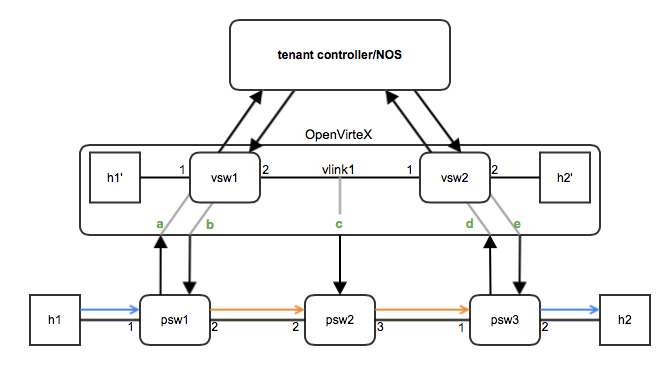
\includegraphics[width=0.7\textwidth]{logo/addr_virt.png}
  \caption{地址虚拟化过程}
  \label{fig:addr-vir}
\end{figure}

虚拟化流程如下:
\begin{enumerate}[a)]
\item PacketIn消息携带VirtualIP,未经修改直接发送给租户控制器
\item 相应的FlowMod匹配VirtualIP,执行的OFAction为将值修改为PhysicalIP。
\item 虚拟链路通过核心侧交换机psw2映射回两跳路径。
\item 目的地边缘的PacketIn与核心网络中的转换行为一致。
\item 虚拟化平台下发与PhysicalIP匹配的FlowMod消息。执行的OFAction为重写回VirtualIP。
\end{enumerate}

转换的过程主要对PacketIn、PacketOut和FlowMod消息的虚拟化与去虚拟化。针对PacketIn消息,由于该消息是来自南向物理交换机,所以消息的处理过程为虚拟化过程,具体的虚拟化过程如图\ref{fig:packetin}所示。首先判断该数据报是否来自边缘侧交换机,如果是,直接查看租户ID和虚拟交换机,如果不是,通过对数据域的匹配,获取租户的ID和虚拟交换机,进而检查该租户的控制器是否以建立连接,如果建立连接,直接将消息发送给租户控制器,否则丢弃。针对L3层的数据报,首先检查PhysicalIP的合理性,在合理的情况下,查看虚拟IP和交换机,并将数据包中的IP地址进行重写。

\begin{figure}[!htb]
  \centering
  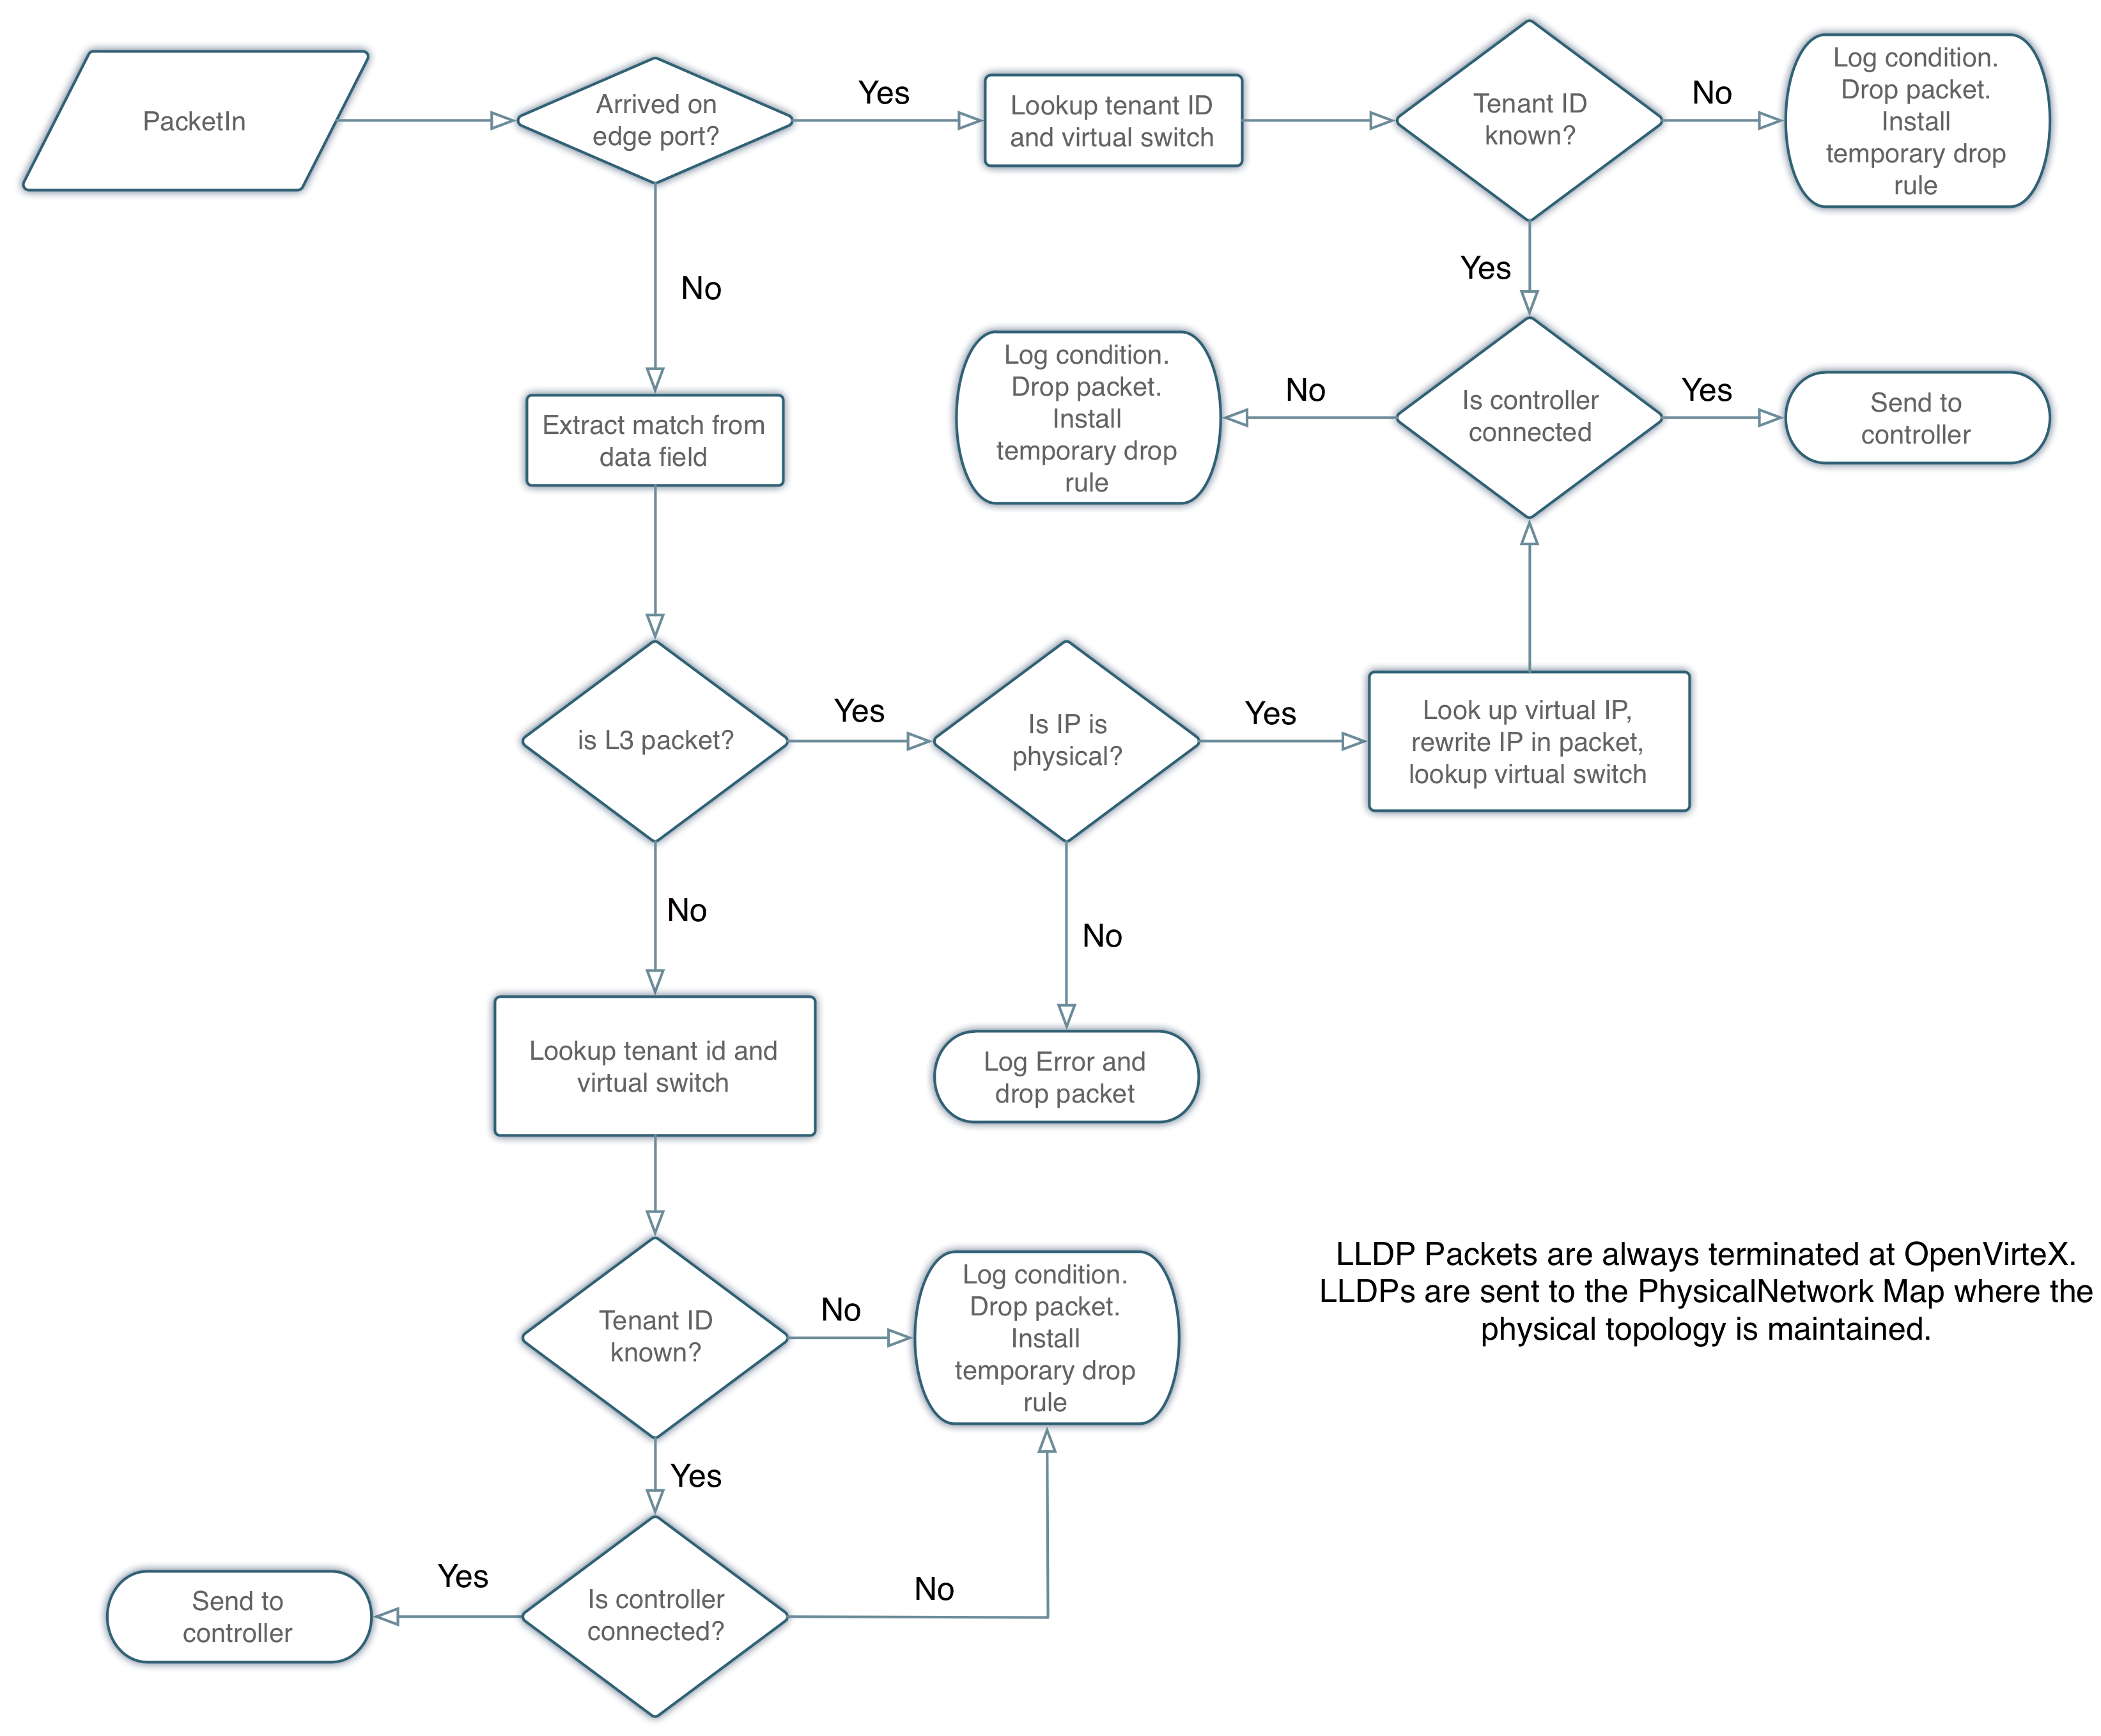
\includegraphics[width=0.7\textwidth]{logo/PacketIn.png}
  \caption{PacketIn虚拟化}
  \label{fig:packetin}
\end{figure}

针对PacketOut消息,由于该消息是由北向租户控制器下发给交换机,所以该消息的处理过程是去虚拟化过程,具体的去虚拟化过程如图\ref{fig:packetout}所示,首先减产bufferID的合理性,进而从data中提取匹配域,重写端口以及bufferID等信息,执行的动作是修改地址为PhysicalIP。

\begin{figure}[!htb]
  \centering
  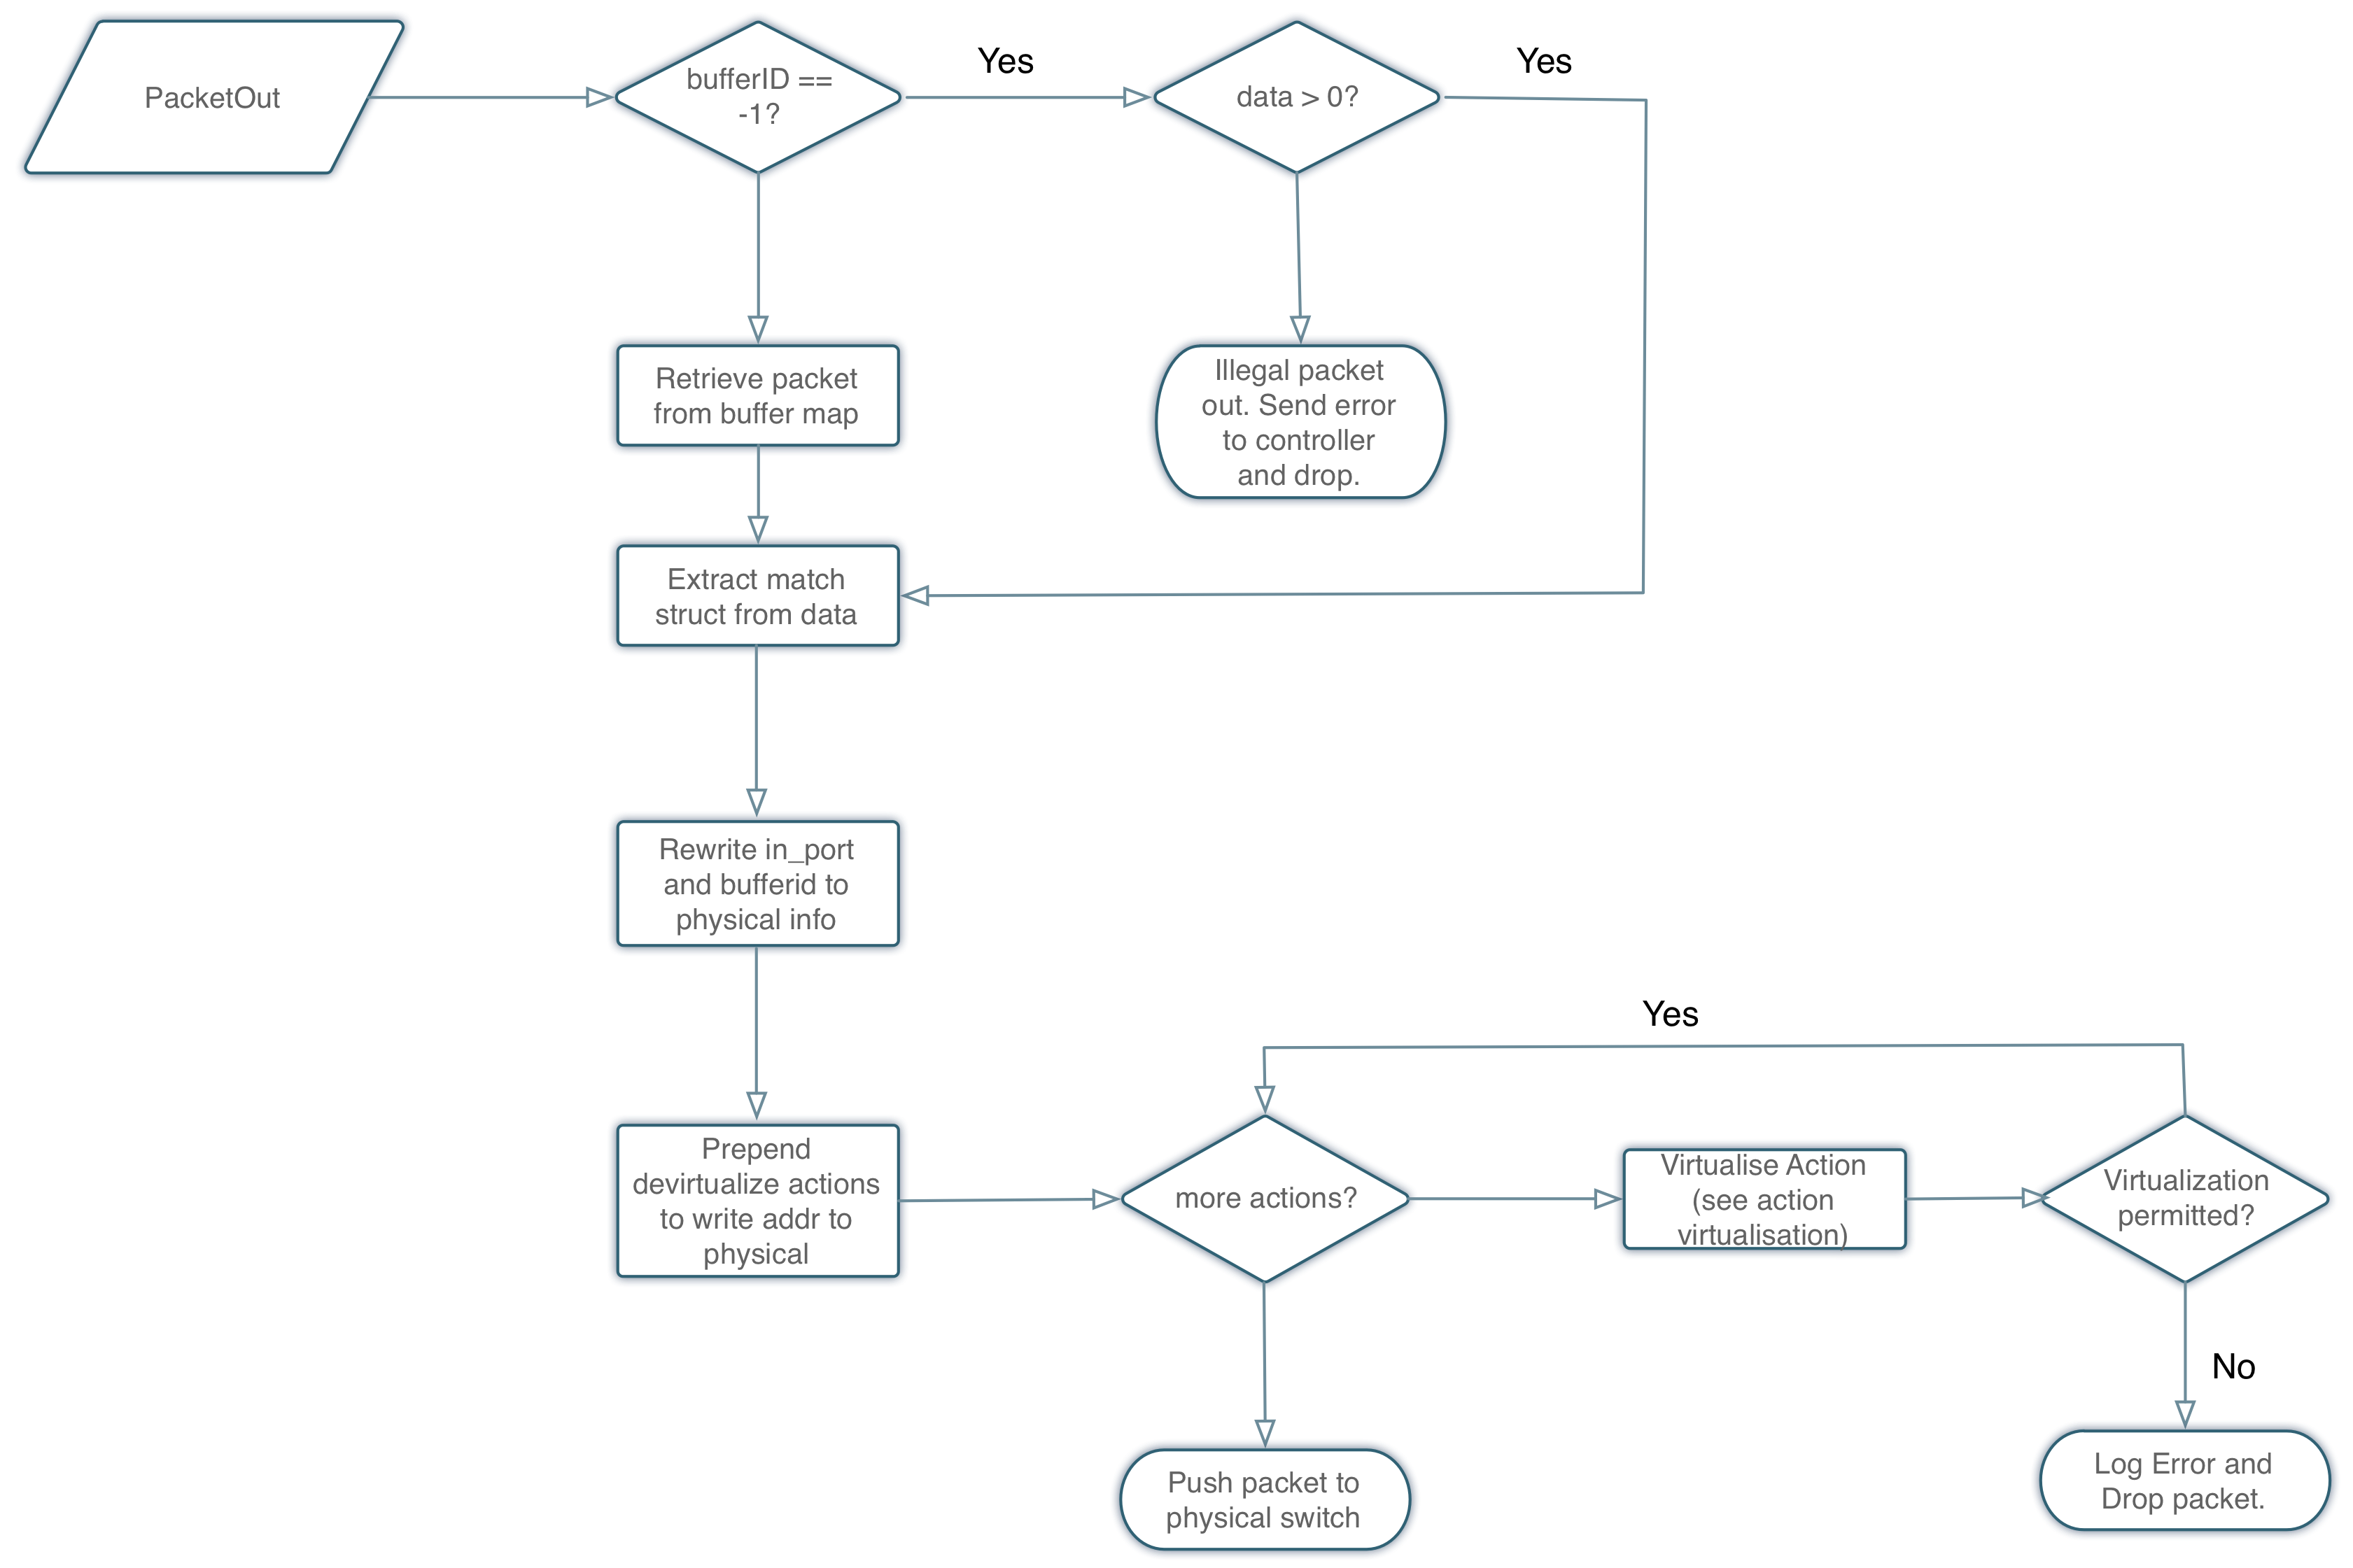
\includegraphics[width=0.7\textwidth]{logo/PacketOut.png}
  \caption{PacketOut去虚拟化}
  \label{fig:packetout}
\end{figure}

针对FlowMod消息,由于该消息是由北向租户控制器发送给交换机,因此,该过程也是一个去虚拟化的过程。首先需要判断该条流是来自入口交换机、出口交换机,还是核心交换机,针对不同的情况进行具体的操作。如果该消息来自出口交换机或者核心交换机,需要将匹配域重写为PhysicalIP,然后,依次将执行的动作重写为物理地址,然后将消息下发给物理交换机。

\begin{figure}[!htb]
  \centering
  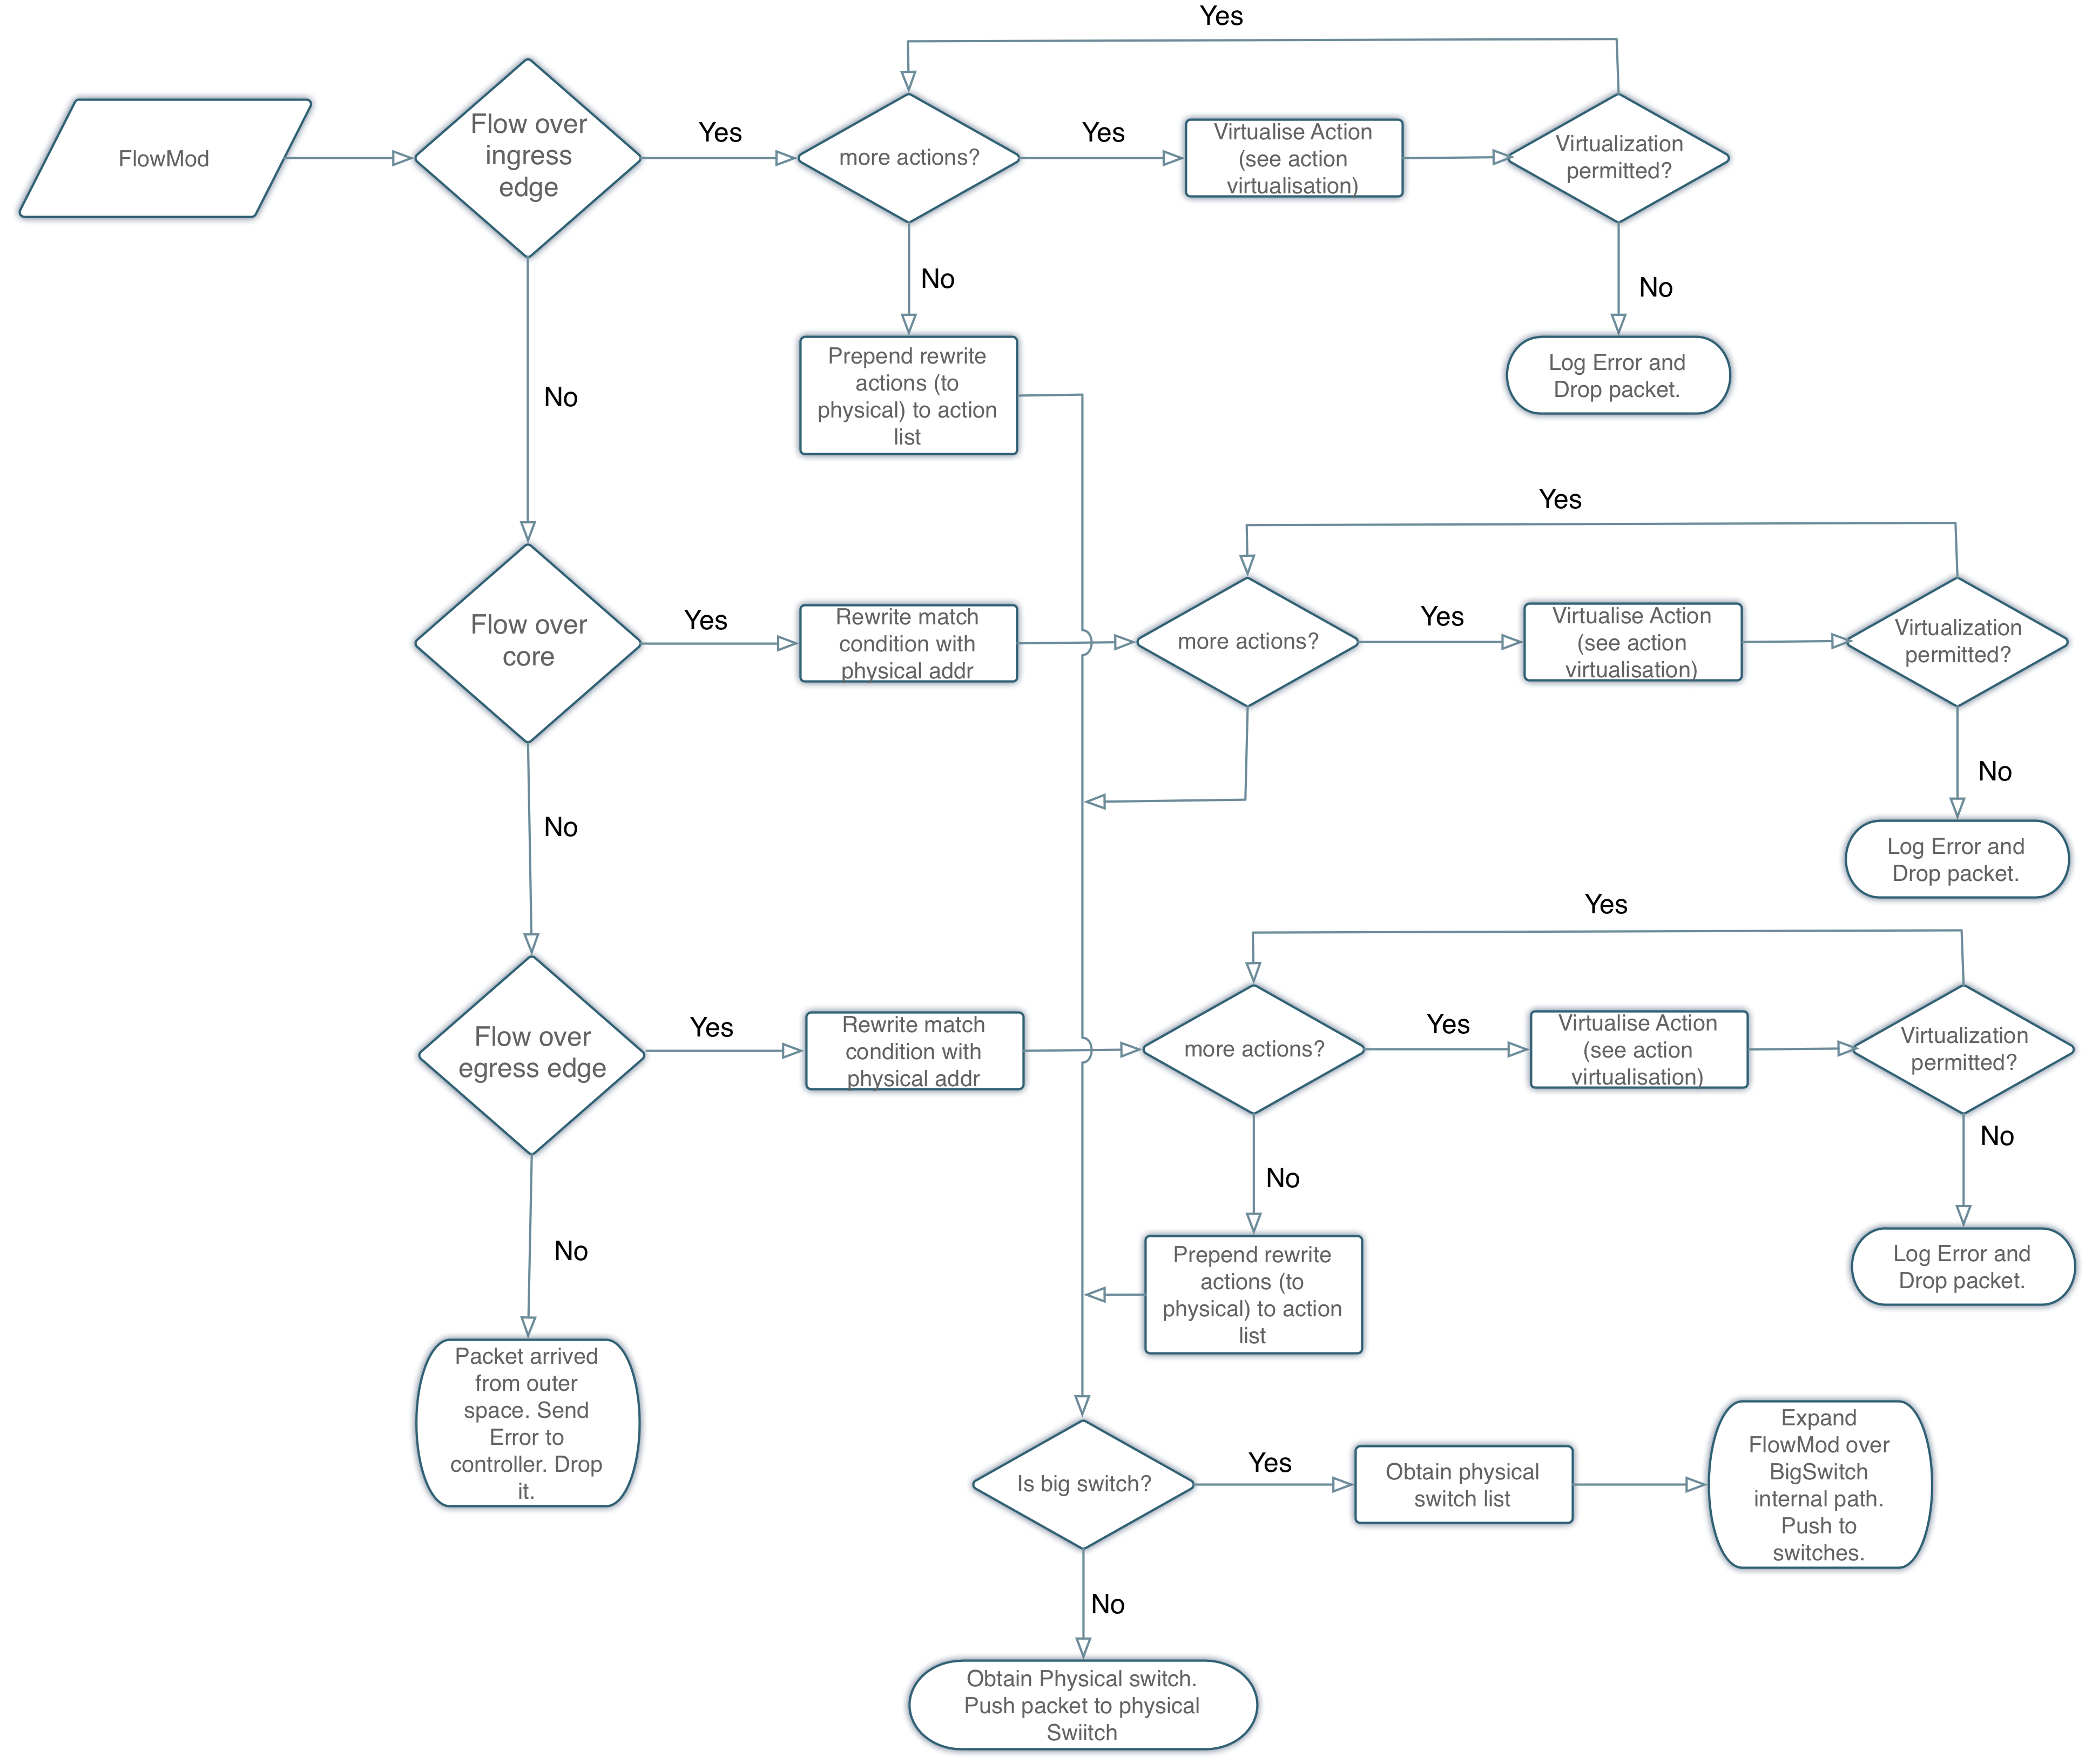
\includegraphics[width=0.7\textwidth]{logo/FlowMod.png}
  \caption{FlowMod虚拟化}
  \label{fig:flowmod}
\end{figure}
\subsection{虚拟网络创建}
针对虚拟网络的创建,本研究中为其封装了API接口\emph{createCustomNetwork},该接口的输入数据为Json格式的物理网络拓扑图,具体的输入信息如下:

\begin{python} 
topo = {
	'subnet':'type:str', #str,虚拟网络的网络地址/位数,例如'192.168.0.0/24'
	'switches':[
		{
			'dpid':'type:str'
		}
	], #物理交换机列表,列表中的每个交换机由dpid标识
	'hosts':[
		{
			'mac':'type:str',
			'port':'type:int',
			'dpid':'type:str'
		}
	], #list,物理主机列表,列表中每条主机信息为dict,存储主机的mac地址、连接物理交换机的dpid和port
	'ctrls':'type:str', #租户控制器信息,包括租户控制器所在IP以及占用的TCP端口,例如'tcp:10.0.0.2:6633'
	'method':'type:str', #请求的函数方法名,
	'routing':{
		'algorithm':'type:str'
	}, #路由算法,例如'spf'
}
\end{python}

进行虚拟网络创建的伪代码如伪代码1所示,主要分4个步骤完成,首先基于租户控制器信息以及创建虚拟网络的子网信息,创建一个逻辑的虚拟网络,返回虚拟网络的ID号;进而基于交换机信息,创建一一对应的虚拟交换机信息;然后对主机信息,依次创建虚拟端口,绑定到特定虚拟交换机,最后,对链路信息,依次创建端口映射,进而对相连接的端口建立虚拟链路。至此,整个虚拟网络创建成功。

\begin{algorithm}[!htb]
    \caption{虚拟网络创建}
    \begin{algorithmic}[1] %每行显示行号
        \Require 物理网络拓扑图,$topo$
        \Ensure 租户虚拟网络ID号,$tenantId$
        \Function {createCustomNetwork}{$topo$}
            \State $ctrls \gets topo['ctrls']$
            \State $subnet \gets topo['subnet']$
            \State $route \gets topo['routing']['algorithm']$
            \State $switches \gets topo['switches']$
            \State $hosts \gets topo['hosts']$
            \State $links \gets topo['links']$
            \State $tenantId \gets createvNetwork(ctrls,subnet)$
            \For{$dpid$ \textbf{in} $switches$}
            	\State $createvSwitch(tenantId, dpid)$
            \EndFor
            \For{$host$ \textbf{in} $hosts$}
            	\State $(vdpid, vport) \gets createvPort(tenantId, host['dpid'],host['port'])$
            	\State $connectvHost(tenantId, vdpid, vport, host['mac'])$
            \EndFor
            \For{$link$ \textbf{in} $links$}
            	\State$(srcdpid, srcport) \gets (ink['src']['dpid'], link['src']['port'])$
            	\State$(dstdpid, dstport) \gets (link['dst']['dpid'], link['dst']['port'])$
            	\State $(srcvdpid, srcvport) \gets createvPort(tenantId, srcdpid, srcport)$
            	\State $(dstvdpid, dstvport) \gets createvPort(tenantId, dstdpid, dstport)$
            	\State $connectvLink(tenantId, srcvdpid, srcvport, dstvdpid, dstvport, route)$
            \EndFor
            \State $startvNetwork(tenantId)$
            \State \Return{$tenantId$}
        \EndFunction
    \end{algorithmic}
\end{algorithm}

\section{通信模块}
通信模块主要实现进程见得异步通信,本文基于消息队列实现,由发送方和接收方组成。发送放主要实现的功能是将需要发送的数据,准确无误的发送至消息队列中,消息队列用于存储通信双方需要传送的数据,直到接收方从队列中读取完成。

发送方的具体实现代码如下:

\begin{python} 
def create():
    pass
class Test(object):
    def __init__():
        pass
        Exception
        sqrt(100)
        a == 100
        b = 10
        c = "sssssss"
        #nihao sdjslk
\end{python}  

接受方具体实现代码如下:

\begin{minted}[linenos=false,fontsize=\scriptsize,bgcolor=bg]{python} 
def create():
    pass
class Test(object):
    def __init__():
        pass
        Exception
        sqrt(100)
        a == 100
        b = 10
        c = "sssss"
        #nihao sdjslk
\end{minted}  
\section{控制器模块}
\subsection{可用带宽测量}
本文基于包对算法,实现细粒度的链路可用带宽的测量,包对技术的核心思想是,连续发送两个背靠背的数据包,由交换机A发送至交换机B,根据两个数据包到达交换机B的时间差,用数据包的长度/时间差,得到精确的链路可用带宽。经测试证明,该方法在低带宽模式下,具有相当精确的测量值。

该技术的实现,要求精确的时间差,对此本文拟定的方案是:首先SDN控制器对交换机下发两条特殊的流表,用于进行带宽测量的数据包的转发工作。对入口交换机下发流表执行的动作是连续两次转发该数据报,从而在链路中产生两个背靠背传输的数据报,对于出口交换机下发流表执行的动作是将数据报转发回控制器。具体如图\ref{fig:spaceband}所示,为了在数据包中存储到达目的交换机的时间,本文对\gls*{OVS}进行源码变更,在匹配到特殊数据包(用于测量带宽的特定数据包,用特殊的IP地址标识)时,对数据包做改动,将数据包IPv6字段替换成当下时间,而后将数据包发送给控制器,控制器从数据报中解析出到达交换机的时间,即可得到背靠背数据包到达目的交换机的时间差,数据包的大小与时间差的比值,即为当前链路的可用带宽。而对于测量用的数据包,本文通过SDN控制器模拟一个满足需求的特定数据包下发给交换机,用于在交换机之间进行传输。

\begin{figure}[!htb]
  \centering
  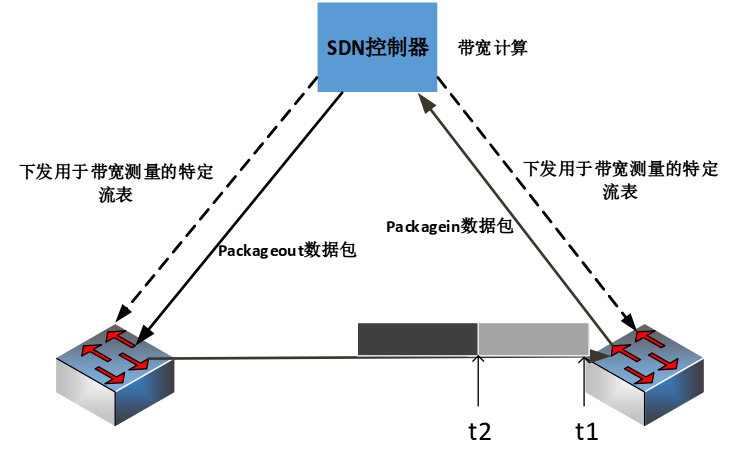
\includegraphics[width=0.7\textwidth]{logo/spaceband.png}
  \caption{链路可用带宽测量模型}
  \label{fig:spaceband}
\end{figure}

对于OVS的开发工作,主要涉及到对特定数据包的修改工作,即将数据包中的IPv6字段替换为当前的时间,具体如伪代码2所示。由伪代码可以看出,本文对特定数据包的要求为源、目的IP均为0,由于该数据包由SDN控制器模拟产出,而且在实际的生活中是不存在的,所以不影响整个系统的运行。

\begin{algorithm}[!htb]
    \caption{OVS为数据包添加当下时间}
    \begin{algorithmic}[1] %每行显示行号
        \Require 数据包,$packet$
        \Ensure 包含当前时间的数据报,$newpacket$
        \Function {modifyIPv6totime}{$packet$}
        	\State $srcip \gets packet.get('srcipv4')$
        	\State $dstip \gets packet.get('dstipv4')$
        	\If{$srcip==0$ \textbf{and} $dstip==0$}
        		\State $localtime \gets time.time$
        		\State $packet.update(ipv6, localtime)$
        	\EndIf
      		\State $newpacket \gets packet$
      		\State \Return{$newpacket$}
        \EndFunction
    \end{algorithmic}
\end{algorithm}

对于控制器端主要开发的功能包括,第一、模拟源、目的IP都为0的IP数据包。第二、为两个交换机下发用于测量带宽的流表。第三、对于控制器接收到的数据包,如果匹配数据包是用来测量可用带宽的,对数据包进行解析,获取时间差,计算当前链路的可用带宽。具体如伪代码3所示。

\begin{algorithm}[!htb]
    \caption{SDN控制器测量可用带宽}
    \begin{algorithmic}[1] %每行显示行号
        \Require 链路的源、目的交换机信息、交换机上报的数据包,$srcswitch,dstswitch,packets$
        \Ensure 当前链路的可用带宽,$bandwidth$
        \Function {add\_flow}{$srcswitch,dstswitch$}
        	\State $srcaction \gets [parser.OFPActionOutput(2),parser.OFPActionOutput(2)]$
        	\State $dstaction \gets [ofproto.OFPPCONTROLLER]$
        	\State $addFlowMod(srcswitch,srcaction)$
        	\State $addFlowMod(dstswitch,dstaction)$
        \EndFunction
        \Function {simulatePacket}{$srcswitch$}
        	\State $pkt \gets packet.Packet()$
        	\State $pkt.update(ipv4(src="0.0.0.0",dst="0.0.0.0"))$
        	\State $sendpacketout(pkt, srcswitch)$
        \EndFunction
         \Function {calculateBandwidth}{$packets$}
         	\State $starttime \gets packets[0].get(ipv6)$
         	\State $endtime \gets packets[1].get(ipv6)$
         	\State $bandwidth \gets (packets[0].size()/(endtime-starttime))$
         	\State \Return{$bandwidth$}
        \EndFunction
    \end{algorithmic}
\end{algorithm}
\subsection{已用带宽测量}
对于已用带宽的测量,本文基于数据包统计的方案实现。由第二章中的表\ref{table:flow}可以看出,流表中具有计数器字段,计数器用于统计流表被匹配的次数,以及匹配的数据包的大小。本文基于此,提出了基于计数器的已用带宽测量,通过统计某段时间内,从交换机某端口发出/接受的数据包数,取平均值进行已用带宽的测量工作,具体实现如伪代码4所示。

\begin{algorithm}[!htb]
    \caption{SDN控制器测量已用带宽}
    \begin{algorithmic}[1] %每行显示行号
        \Require 链路的源、目的交换机信息,以及交换机的端口号,$src_switch,src_port,dst_switch,dst_port$
        \Ensure 当前链路的已用,$bandwidth$
        \Function {get\_counters}{$srcswitch,srcport, dstswitch,dstport$}
        	\State $inputBytes \gets getCounters(srcswitch, inport=srcport)$
        	\State $outputBytes \gets getCounters(srcswitch, outport=srcport)$
        	\State $allBytes \gets (inputBytes+outputBytes)$
        	\State \Return{$allBytes$}
        \EndFunction
        \Function {calculateBandwidth}{$srcswitch,srcport, dstswitch,dstport$}
        	\State $bytes1 \gets getcounters(srcswitch,srcport, dstswitch,dstport)$
        	\State $time.sleep(sometime)$
        	\State $bytes2 \gets getcounters(srcswitch,srcport, dstswitch,dstport)$
        	\State $bandwidth \gets ((bytes2-bytes1)/sometime)$
         	\State \Return{$bandwidth$}
        \EndFunction
    \end{algorithmic}
\end{algorithm}
\subsection{时延测量}
时延的测量,本研究采用最基本的基于三点的测量方法。即控制器与两台交换机组成最小的测量单元,分别测出控制器到交换机的时延以及三边的总时延,做差值即为链路的时延。模型如图\ref{fig:delay}所示,图中链路的时延即为t3-(t1+t2)/2。

\begin{figure}[!htb]
  \centering
  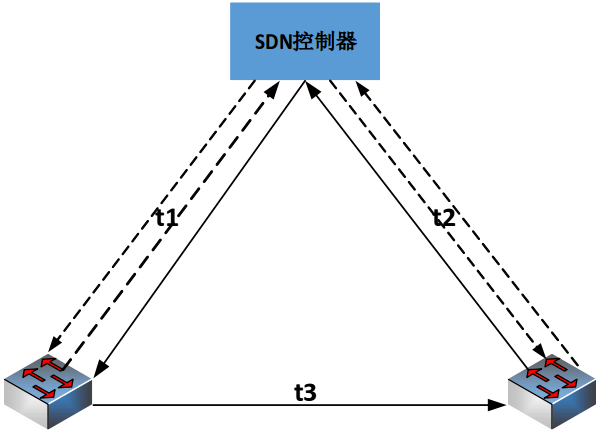
\includegraphics[width=0.7\textwidth]{logo/delay.png}
  \caption{链路时延测量模型}
  \label{fig:delay}
\end{figure}

具体实现如伪代码5所示。
\subsection{定制化流表下发}
\section{GUI模块}
\subsection{拓扑显示}
\subsection{虚拟网络创建}
\subsection{带宽时延查询}
\subsection{定制化流表下发}
\section{本章小结}